\documentclass[]{article}
\usepackage[english]{babel}
\usepackage[margin=0.8in]{geometry}
\usepackage{graphicx}
\usepackage{caption}
\usepackage{titling}
\begin{document}
\title{
  Project management report \\
 \Large{ DynamoDB and embedded data}
}
\author{Embedded data handling in .NET with Amazon DynamoDB} %used author space for creating a subtitle, A little unhortodox ik lol
\maketitle
	\section{Instructions}\label{intro}
	The instructions of the project are to create an application that would automatically insert embedded river-type data within a database created through the AWS DynamoDB service.\\
	The application also has allow the database to be queried through a graphical interface and display the results on the screen.
	\section{Classes Design}
	The approach for using the classes was to use each one for creating a resource or interacting with a service not already present.
	\begin{figure}[h!]
		\centering
		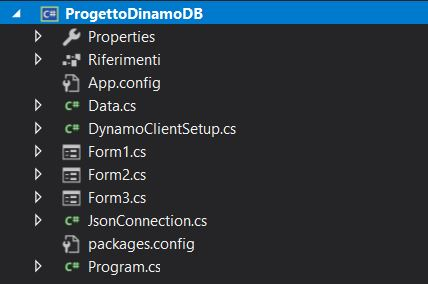
\includegraphics[width=0.5\columnwidth]{ProgettoDinamoDBclassi.JPG}
		\label{figClasses}
		\caption*{The scheme of the project classes}
	\end{figure}\\
	The project is based mainly on the "DynamoClientSetup" class, which is needed to obtain and enter data into the Database, and the Data class, which is a class that contains parameters for everything that might be useful for river controls.
	The properties recorded are, in addition to the value of the measurement and an identifier for it (Time Hash), the values of light, temperature, humidity, and water level.\\
	This data is collected through an Arduino, which provides it through a Json to the program C\#, which checks every 5 seconds to see if there is new data input and, if so, it is entered into the Database.
	\pagebreak
	\section{The program functioning}
	The interface is based on three forms:
		\begin{figure}[h!]
		  \centering
		  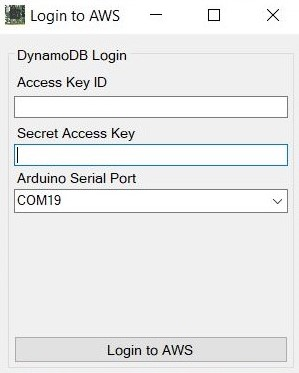
\includegraphics[width=0.25\columnwidth]{Login.JPG}
		  \label{fig1}
		  \caption*{The login interface, that allows to log with our credentials and select the Arduino COM's port}
	\end{figure}
	\begin{figure}[h!]
			\centering
			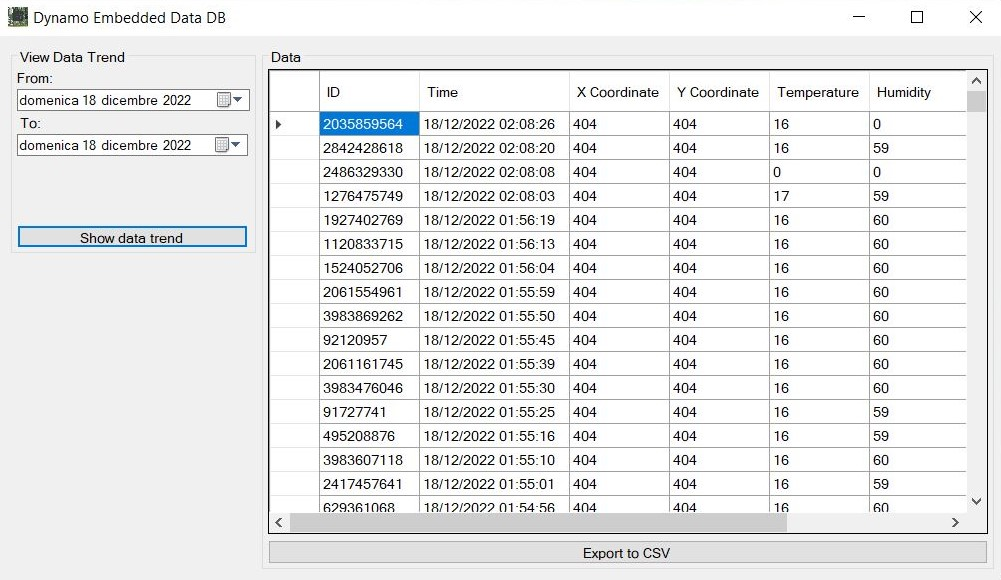
\includegraphics[width=0.5\columnwidth]{Management.JPG}
			\label{fig2}
			\caption*{The daily data management screen}
	\end{figure}
	\begin{figure}[h!]
			\centering
			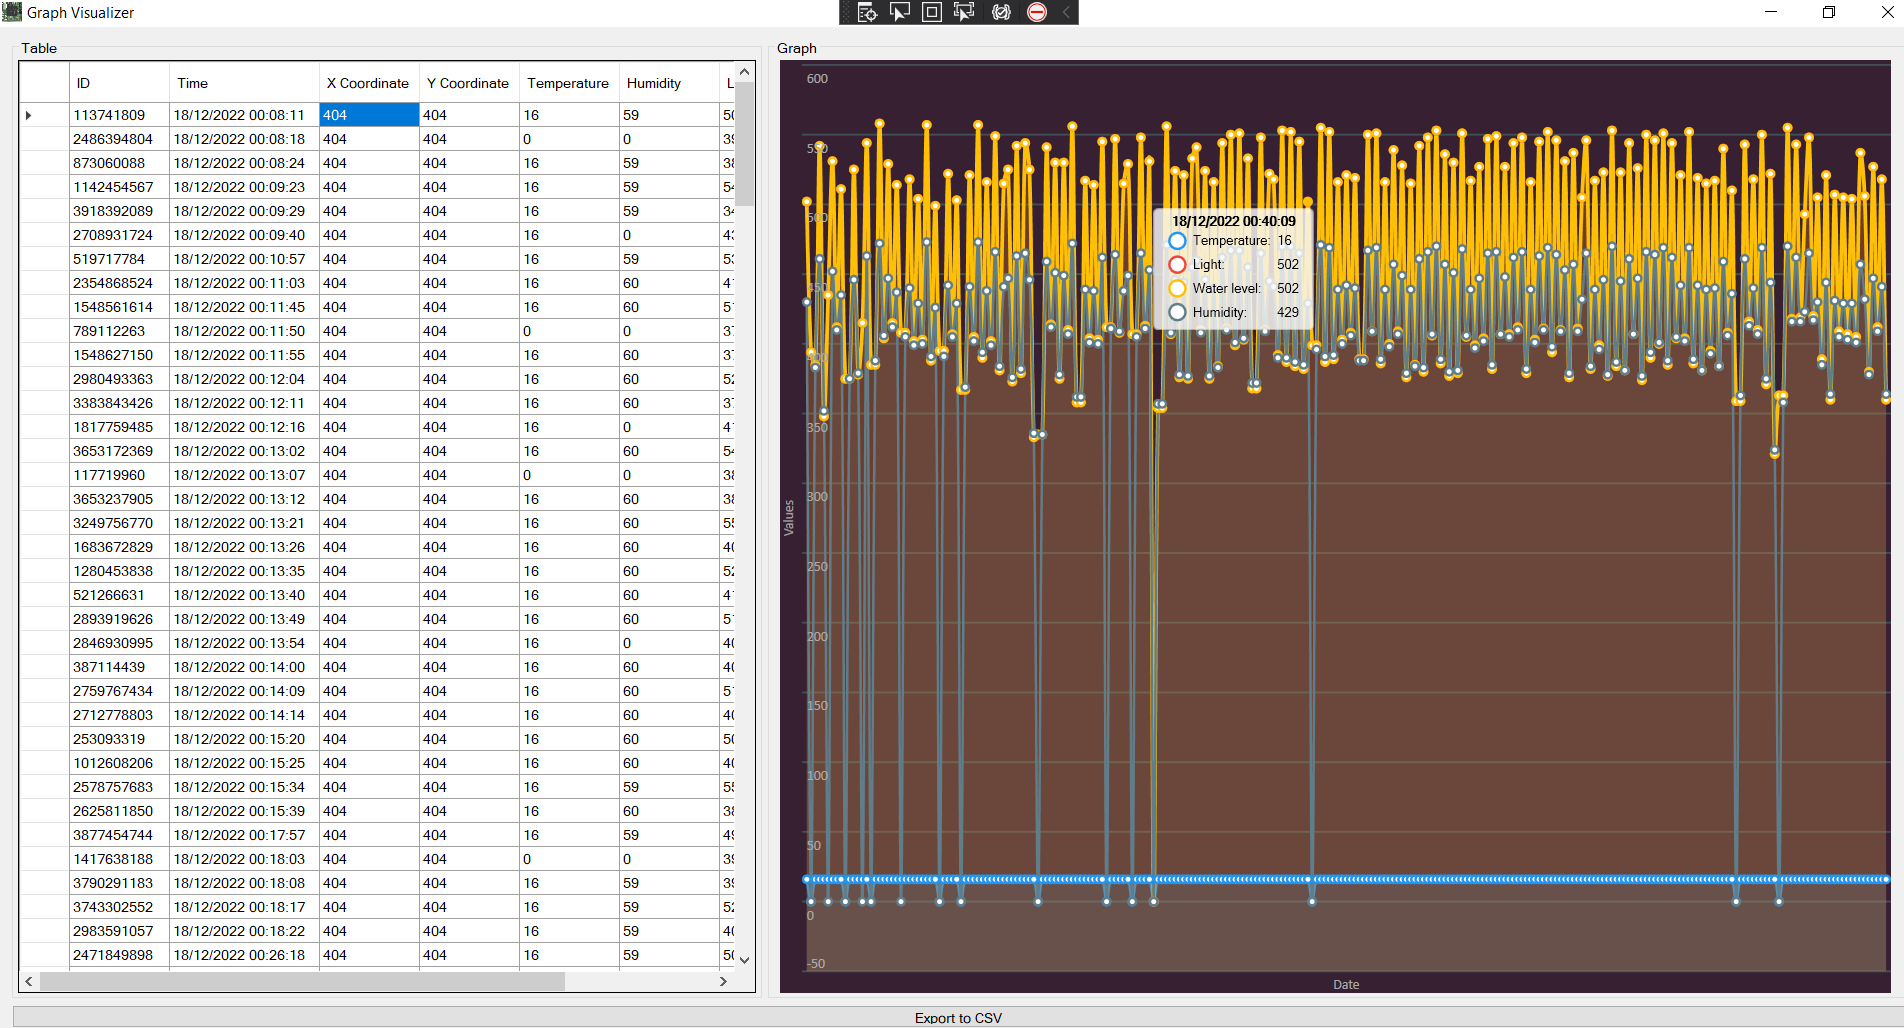
\includegraphics[width=0.5\columnwidth]{Archive.png}
			\caption*{The data trend screen, that allows you to see the Data retrieved in a selected time period}
			\label{fig3}
	\end{figure}
	\pagebreak
	\section{Encountered issues}
	There were many problems encountered, but the main ones were two:
	\begin{itemize}
	\item The first was getting DynamoDB to communicate with the C\# program. The documentation is lacking and sometimes contradictory, which made it particularly difficult to figure out what to do, and one often had to fumble around, succeeding only after many attempts, and it could have been done in much less time if there had been proper documentation and tutorials.
	\item The second was reading from serial and interpreting the documents, read as json, into c\# classes. Here it was difficult to figure out how to do this, and even the Microsoft documentation, though always correct, was often lacking details needed to be able to work.
	\end{itemize}	
	\section{Conclusions}
	DynamoDB has proven to be a very powerful, though certainly unconventional, tool, and the possibilities for use are truly vast.\\
	While this service is not without flaws, it proved to be truly functional and suitable for the project, which allowed us to gain new skills, both with Arduino, Json and DynamoDB, that will surely come in handy in the future and can be reused for new projects.
\end{document}